%!Tex Root = ../Vorlage_Praesentation.tex
% ./Packete.tex
% ./Design.tex
% ./Deklarationen.tex
% ./Kapitel2.tex


\if\hide0\section{Kapitel 1}\fi

\begin{frame}[label={kapitel1}]{Kapitel 1}{Beispiele für Custom Block Environments}
  \begin{custom}{Random}
    random text
  \end{custom}

  \begin{acustom}{Random}
    random text
  \end{acustom}
\end{frame}

\begin{frame}{Kapitel 1}{Beispiele für Custom Block Environments}
  \begin{custom}{Random}
    random text
  \end{custom}

  \begin{acustom}{Random}
    random text
  \end{acustom}
\end{frame}

\begin{frame}{Kapitel 1}{Beispiele für Block Environments}
  % https://latex-beamer.com/tutorials/blocks/
  \begin{block}{Wichtiger Bereich}
    random text
  \end{block}

  \begin{exampleblock}{Wichtiges Beispiel}
    random text
  \end{exampleblock}

  \begin{alertblock}{Wichtiges Text}
    random text
  \end{alertblock}
\end{frame}

\begin{frame}{Kapitel 1}{Beispiele für weitere Custom Theorem Environments}
  \begin{customtheorem}[Wichtiges Custom Theorem]
    random text
  \end{customtheorem}

  \begin{subcustomtheorem}[Wichtiges Sub Custom Theorem]
    random text
  \end{subcustomtheorem}

  \begin{ocustomtheorem}[Wichtiges Custom Theorem]
    random text
  \end{ocustomtheorem}
\end{frame}

\begin{frame}{Kapitel 1}{Beispiele für Theorem Environments}
  \begin{theorem}[Wichtiges Theorem]
    random text
  \end{theorem}

  \begin{corollary}[Wichtiges Korrolar]
    random text
  \end{corollary}

  \begin{lemma}[Wichtiges Lemma]
    random text
  \end{lemma}

  \begin{proof}[Wichtiger Beweis]
    random text
  \end{proof}
\end{frame}

\if\hide0\section{Kapitel 2}\fi

\begin{frame}[label={kapitel2}]{Kapitel 2}{Beispiele für weitere Theorem Environments}

  \begin{definition}[test]
    random text
  \end{definition}

  \begin{definitions}[test]
    random text
  \end{definitions}

  \begin{fact}[test]
    random text
  \end{fact}

  \begin{example}[test]
    ist im Gegensatz zu exampleblock durchnummeriert
  \end{example}
\end{frame}

\begin{frame}{Kapitel 2}{Beispiele für weitere Theorem Environments}
  \begin{examples}[test]
    random text
  \end{examples}
\end{frame}

\begin{frame}{Kapitel 2}{Beispiel für Tabelle}
  \scriptsize
  \begin{table}[H]
    \center
    \begin{NiceTabular}{X[1,c]X[2,l]}[rules/color=PrimaryColor] % {\linewidth}{|C|C|L|L|}
      \CodeBefore
      \chessboardcolors{white}{BoxColor}
      \rowcolor{PrimaryColor}{1}
      \Body
      \textcolor{white}{Spalte 1} & \textcolor{white}{Spalte 2} \\
      \scripttt{row1} & \alert{Beschreibung} für \scripttt{row1}. \\
      \scripttt{row2} & \aalert{Beschreibung} für \scripttt{row2}. \\
      \bottomrule
    \end{NiceTabular}
    \caption{Beispiel.}
  \end{table}
\end{frame}

\begin{frame}{Kapitel 2}{Beispiel für Diagram}
  \begin{figure}
    \begin{transformation}[0.2][0.2][0.5]
      {\dq}{4}\enspace {*}\enspace {2}{\dq}
      \arrowxx{Aktion 1}{Aktion 2}
      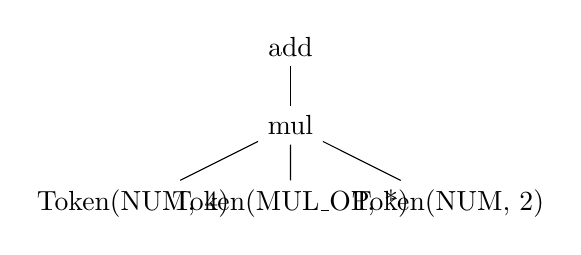
\begin{tikzpicture}[auto, align=center, sibling distance=2cm, level distance=1cm, baseline=(current  bounding  box.center)]
        \node {\tinytt{add}}
        child {node {\tinytt{mul}}
          child {node {\tinytt{Token(NUM, \dq 4\dq)}}}
          child {node {\tinytt{Token(MUL\_OP, \dq *\dq)}}}
          child {node {\tinytt{Token(NUM, \dq 2\dq)}}}};
      \end{tikzpicture}
    \end{transformation}
    \caption{Untertitel.}
  \end{figure}
\end{frame}

\begin{frame}{Kapitel 2}{Weiteres Beispiel für Diagram}
  \begin{equation}
    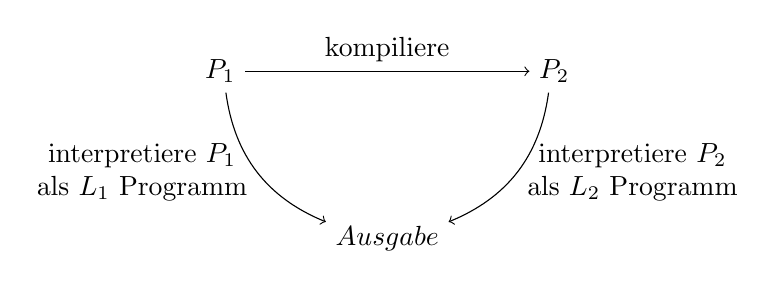
\begin{tikzpicture}[auto, baseline=(current  bounding  box.center)]
      \node (program1) at (135:3) {$P_{1}$};
      \node (program2) at (45:3) {$P_{2}$};
      \node (output)  at (270:0) {$Ausgabe$};

      % https://tex.stackexchange.com/questions/24372/how-to-add-newline-within-node-using-tikz
      \draw[->] (program1) to node[above] {kompiliere} (program2);
      \draw[->] (program1) to[bend right] node[left, align=center] {interpretiere $P_{1}$\\ als $L_{1}$ Programm} (output);
      \draw[->] (program2) to[bend left] node[right, align=center] {interpretiere $P_{2}$\\ als $L_{2}$ Programm} (output);
    \end{tikzpicture}
  \end{equation}
\end{frame}
